\documentclass{article}
\usepackage{amsmath}
\usepackage{graphicx}
\usepackage{color}
\usepackage{booktabs}
\usepackage{multirow}
\usepackage{rotating}
\usepackage[margin=2cm]{geometry}
\DeclareGraphicsRule{*}{eps}{*}{}
\renewcommand{\baselinestretch}{1.5}

\begin{document}

    \begin{center}

        {\Large \bf Talk on 2011-05-16}
    \end{center}

    \section{The information for 2 Genes}
    For the simulation study, we choose two genes from the GWAS study: RBJ and GRPC5B which are two candidate genes for the BMI. After carefully checking the data, the LD and MAF information for the two genes are listed in the following tables:\\
    
    \begin{figure}[htbp]
        \centering
        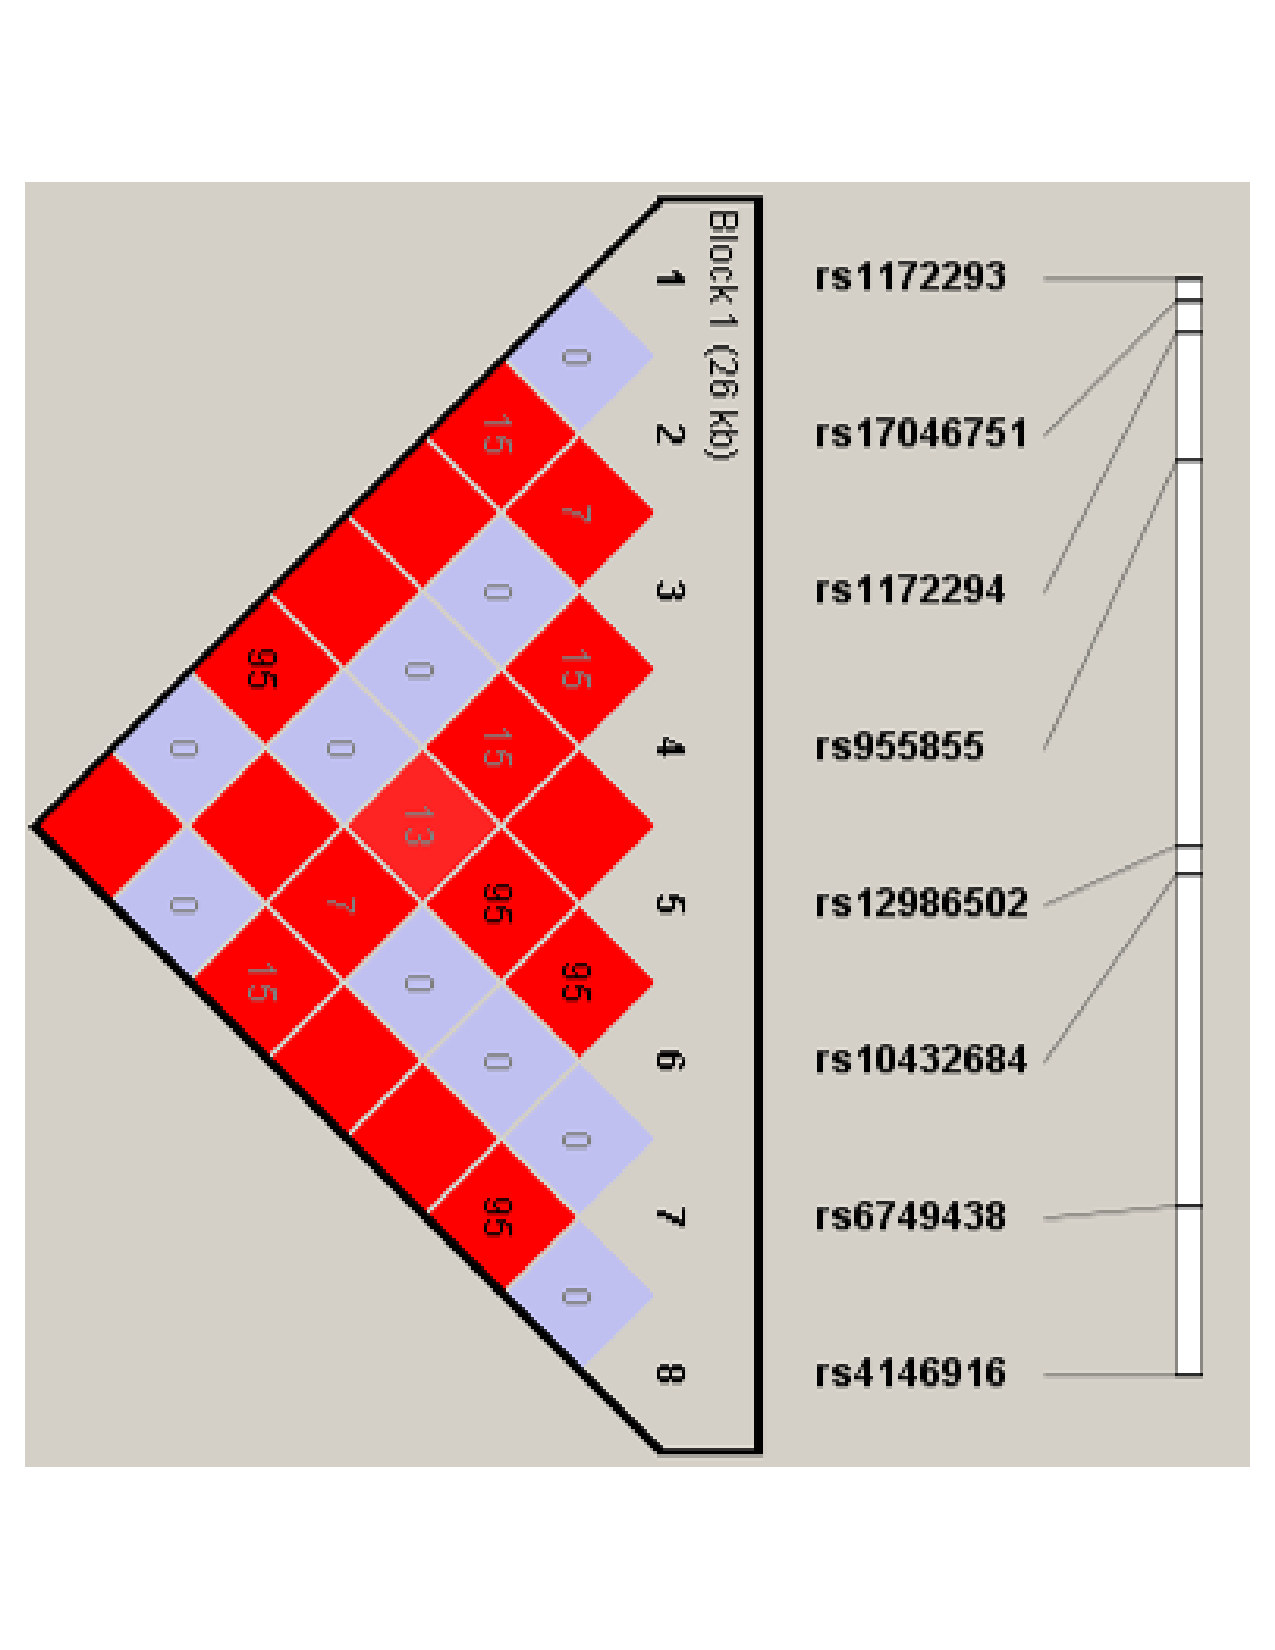
\includegraphics[scale=0.4,angle=90]{RBJ}
        \caption{LD pattern for Gene RBJ}
    \end{figure}

    \begin{table}[htbp]
        \centering
        \caption{The LD and MAF information for Gene RBJ}
        \begin{tabular}{c|cccccccc}
            \hline
            SNP & 1&	2&	3&	4&	5&	6&	7&	8\\
            \hline
            LD &0.588 &	0.159& 	0.126 &	0.588 &	0.588 &	0.565 &	0.159 &	0.588\\
            MAF &0.115 &	0.062 &	0.482 &	0.115 &	0.115 &	0.119 	&0.062& 	0.115\\
            \hline
        \end{tabular}
    \end{table}
    
    \begin{figure}[htbp]
        \centering
        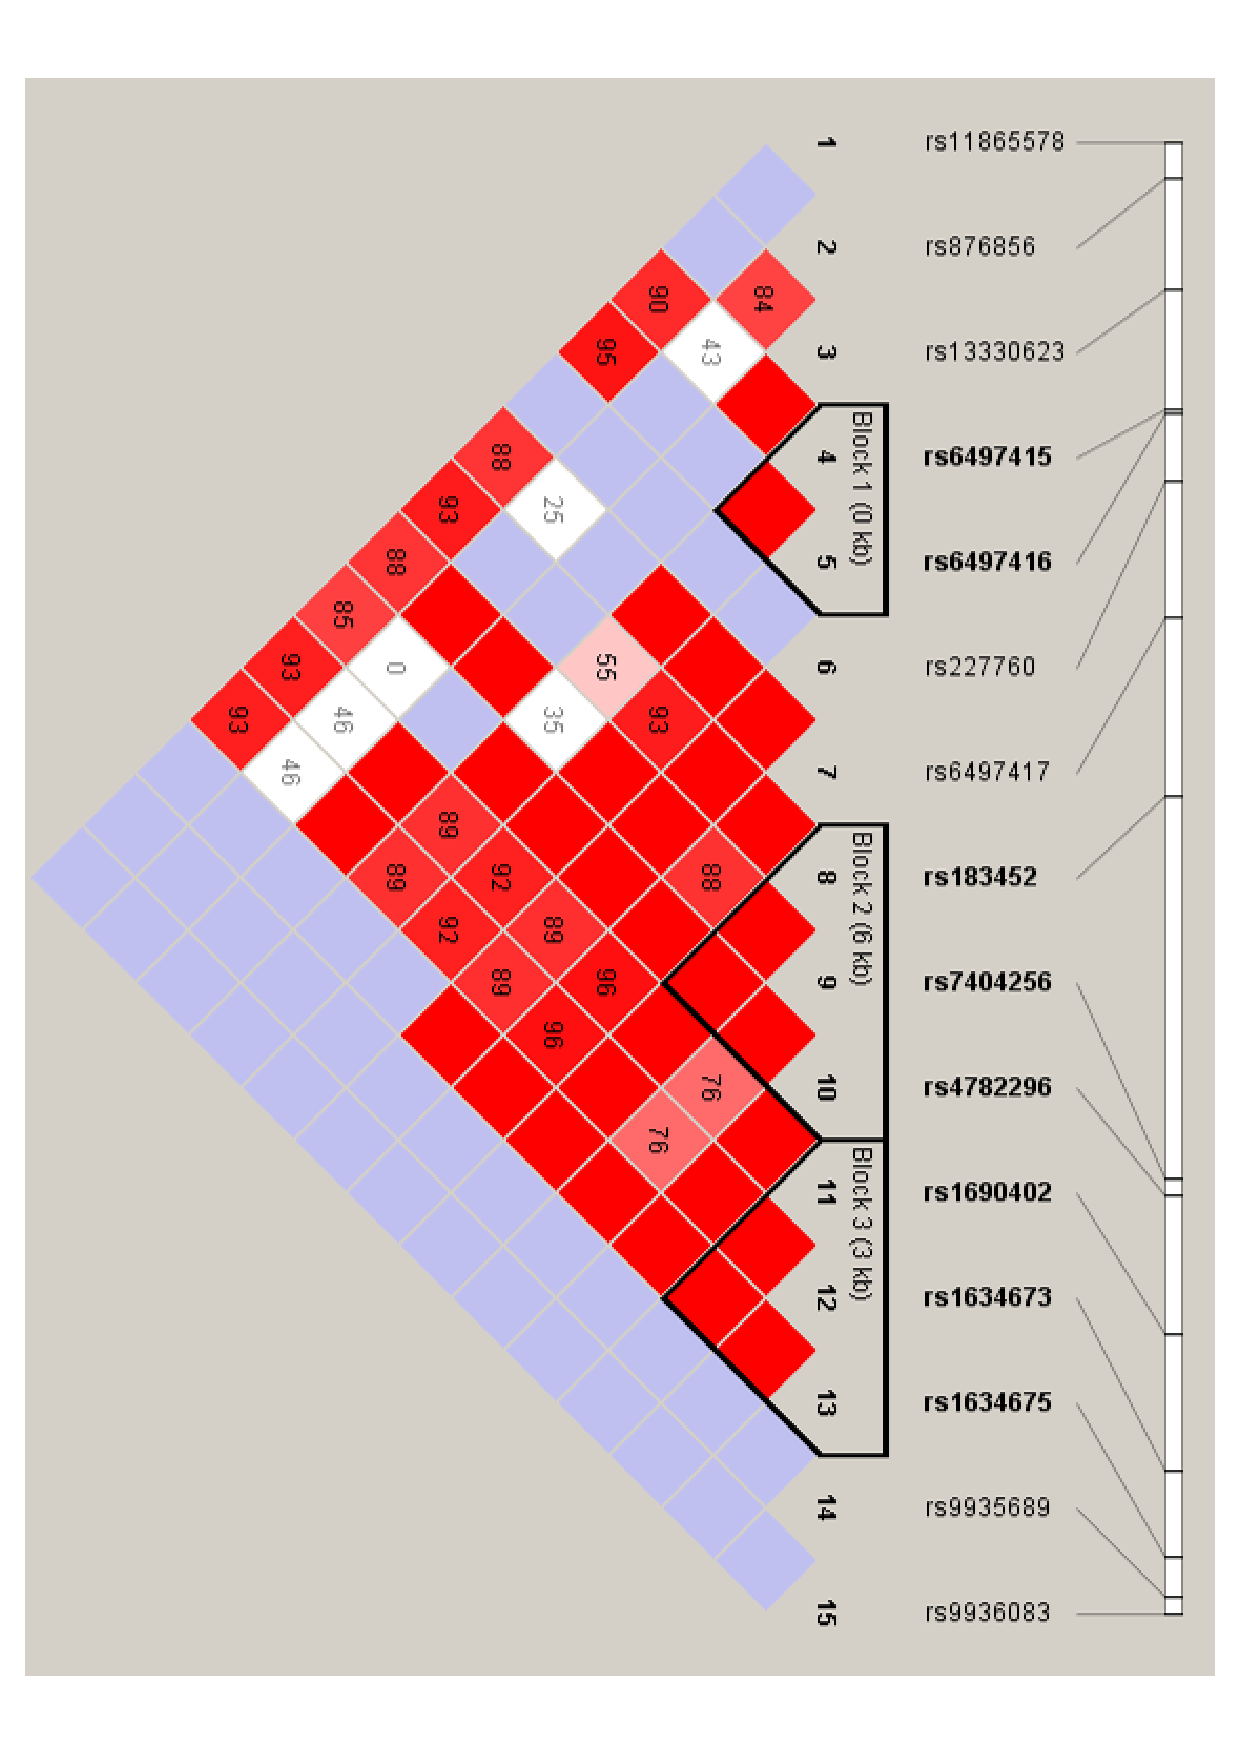
\includegraphics[scale=0.6,angle=90]{GPRC5B}
        \caption{LD pattern for Gene GRPC5B}
    \end{figure}

    \begin{table}[htbp]
        \centering
        \caption{The LD and MAF information for Gene GRPC5B}
        \begin{tabular}{c|ccccccccccccccc}
            \hline
            SNP &1	&2	&3	&4	&5	&6	&7	&8	&9	&10	&11	&12	&13	&14	&15\\
            \hline
            LD  &0.186 &0.050 	&0.065 	&0.194 	&0.197 	&0.136 	&0.259 	&0.262 	&0.230 	&0.206 	&0.285 	&0.285 	&0.138 	&0 	&0\\
            MAF &0.146 &0.066 	&0.044 	&0.195 	&0.143 	&0.159 	&0.460 	&0.336 	&0.482 	&0.371 	&0.394 	&0.394 	&0.155 	&0.004 	&0.005\\
            \hline
        \end{tabular}
    \end{table}

    Based on the information listed above, I set a SNP has high LD with other SNP if its LD $>0.18$ and a common SNP is defined as a SNP whose MAF $>0.2$. Based on the threshold, we eventually pick 3 SNP from each gene as they have different LD MAF combination.
        \begin{table}[htbp]
        \centering
        \caption{The Casual SNP picked up in the two genes}
        \begin{tabular}{cc|cc}
            \hline
            \multicolumn{2}{c}{RBJ}&\multicolumn{2}{c}{GRPC5B}\\
            \hline
            SNP 1 & H, R &SNP 5&H, R\\
            SNP 2& L,R&SNP 6&L,R\\
            SNP 3&L, C &SNP 8& H, C \\
            \hline
        \end{tabular}
    \end{table}

    \section{Simulation Plan}

    We try to investigate the power of our method and other 2 methods (PCA and PLS) though 5 models.\\
    M1: $Y=0.2\times(\theta_{11}+\theta_{21})+\epsilon$\\
    M2: $Y=0.15\times(\theta_{11}\theta_{12}+\theta_{21}\theta_{22})+\epsilon$\\
    M3: $Y=0.15\times(\theta_{11}+\theta_{12}\theta_{22})+\epsilon$\\
    M4: $Y=0.15\times(\theta_{11}+\theta_{12}\theta_{22}+\theta_{21}\theta_{22})+\epsilon$\\
    M5: $Y=0.2\times(\theta_{11}\theta_{21}+\theta_{12}\theta_{22})+\epsilon$\\
    where the Y is the phenotype and $\theta_{ij}$ is the indicator for $jth$ SNP from the $ith$ Gene.

    \section{Result analysis}
    \subsection{Model 1: $Y=0.2\times(\theta_{11}+\theta_{21})+\epsilon$}    
        \begin{figure}[htbp]
            \centering
            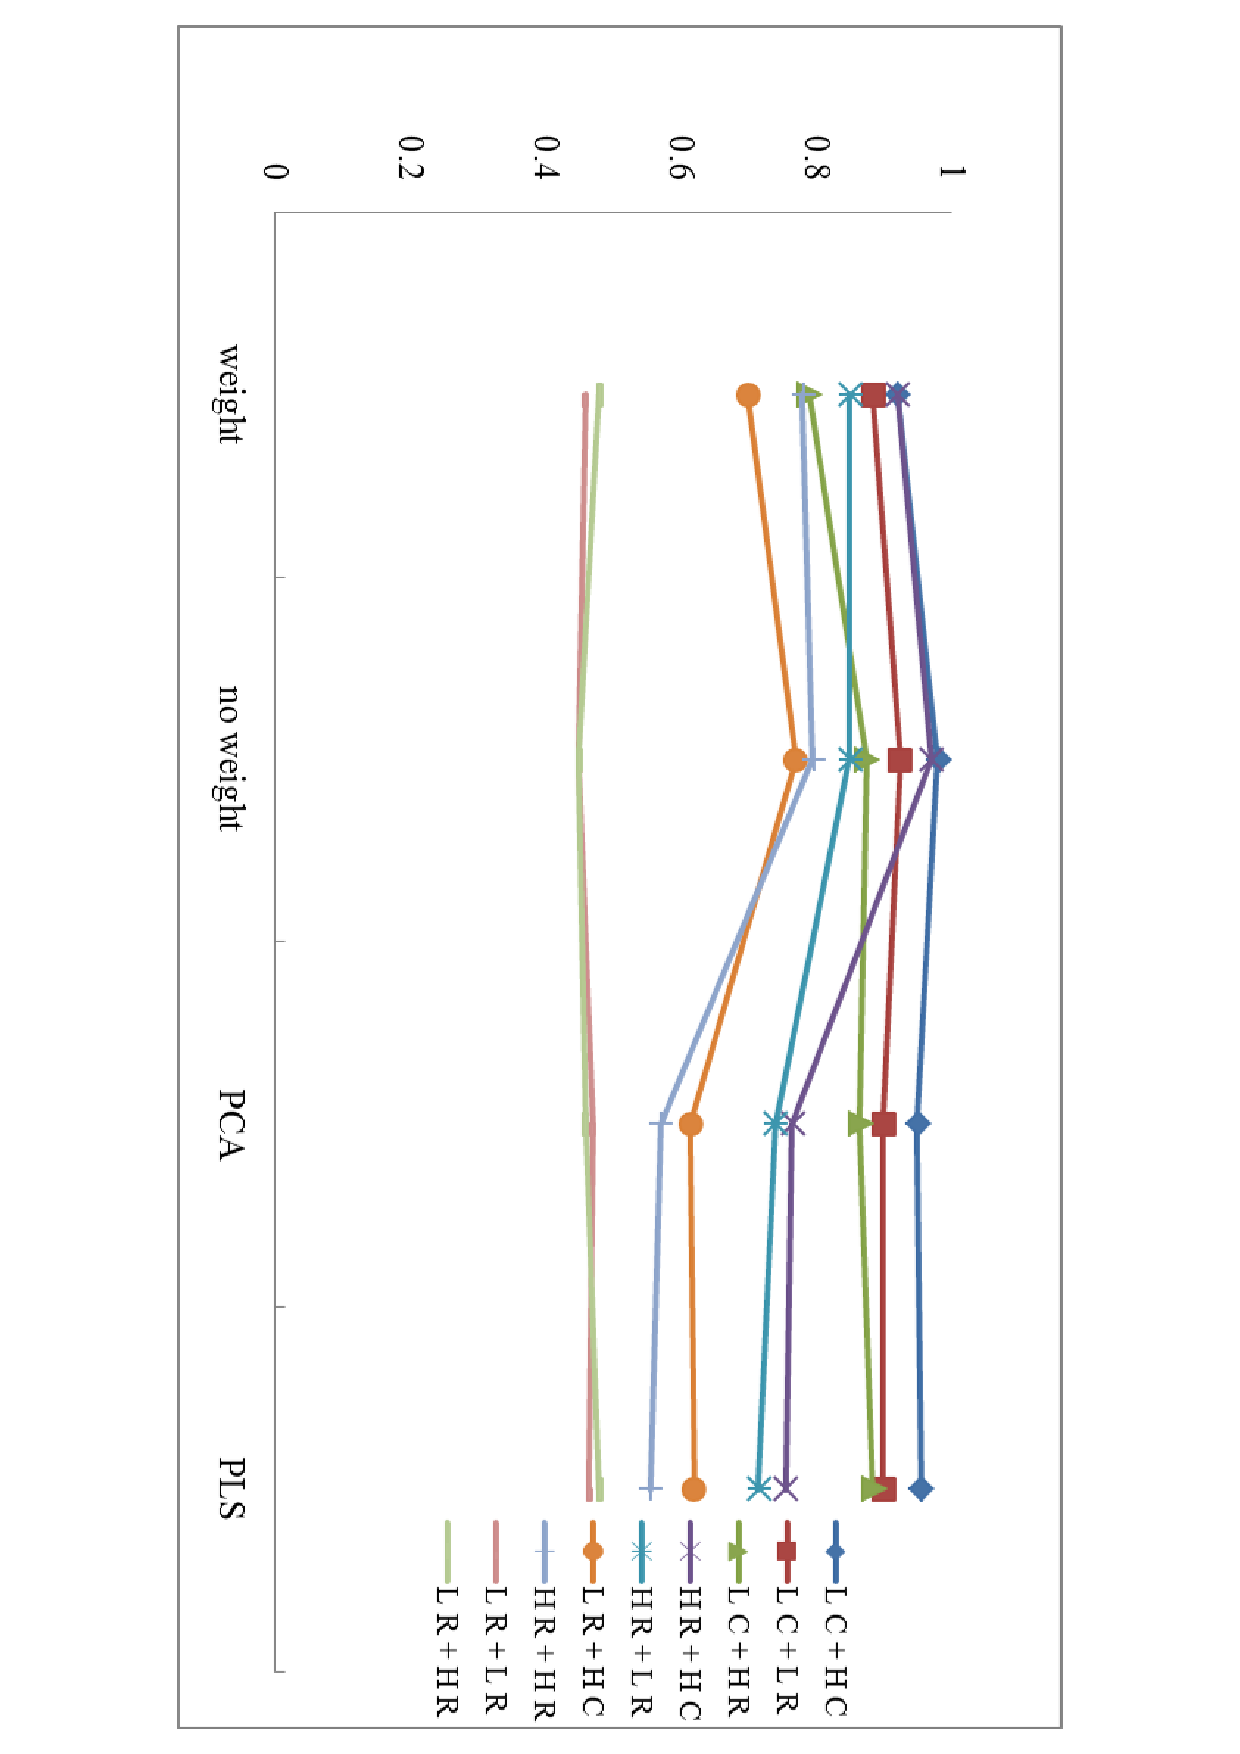
\includegraphics[scale=0.5,angle=90,trim=70 0 70 0, clip=true]{Model1}
            \caption{ALL combinations for Model 1}
        \end{figure}
        Model 1 is an additive model. From the figure we can see that the allele freq. seems more important than the LD pattern and the type of $\theta_{11}$ is more important than the type of $\theta_{21}$. If we just check $\theta_{11}$, i.e., the type of $\theta_{21}$ is the same, we can see that power of different type is $P_{L,C}>P_{H,R}>P_{L,R}$. Similar to $\theta_{11}$, under the same type of $\theta_{11}$, the power for different $\theta_{21}$ is $P_{H,C}>P_{L,R}>P_{H,R}$. (\textcolor{red}{I don't understand why here for $\theta_{21}$, the LR type would give a more strong power than HR while in $\theta_{11}$, the power for HR is more stronger and make more sense, I have double checked it for several times.})

        SNP 3 in Gene RBJ (whose type is L,C ) is a very strong signal to be detect so when it shows up, the power is very strong. So the top 3 all involved. The following power is for the case where $\theta_{11}$ is H,R, but when $\theta_{21}$ is H,R, the power is much lower, so the combination of LR+HC is better than the combination of HR+LR.

        For most cases in model 1, no weight even performs better than the weighted version. The only exception is when the $\theta_{11}$ and $\theta_{21}$ have the RR allele freq. combination. But for me, the different is not significant.

    \subsection{Model 2: $Y=0.15\times(\theta_{11}\theta_{12}+\theta_{21}\theta_{22})+\epsilon$}
    
        \begin{figure}[htbp]
            \centering
            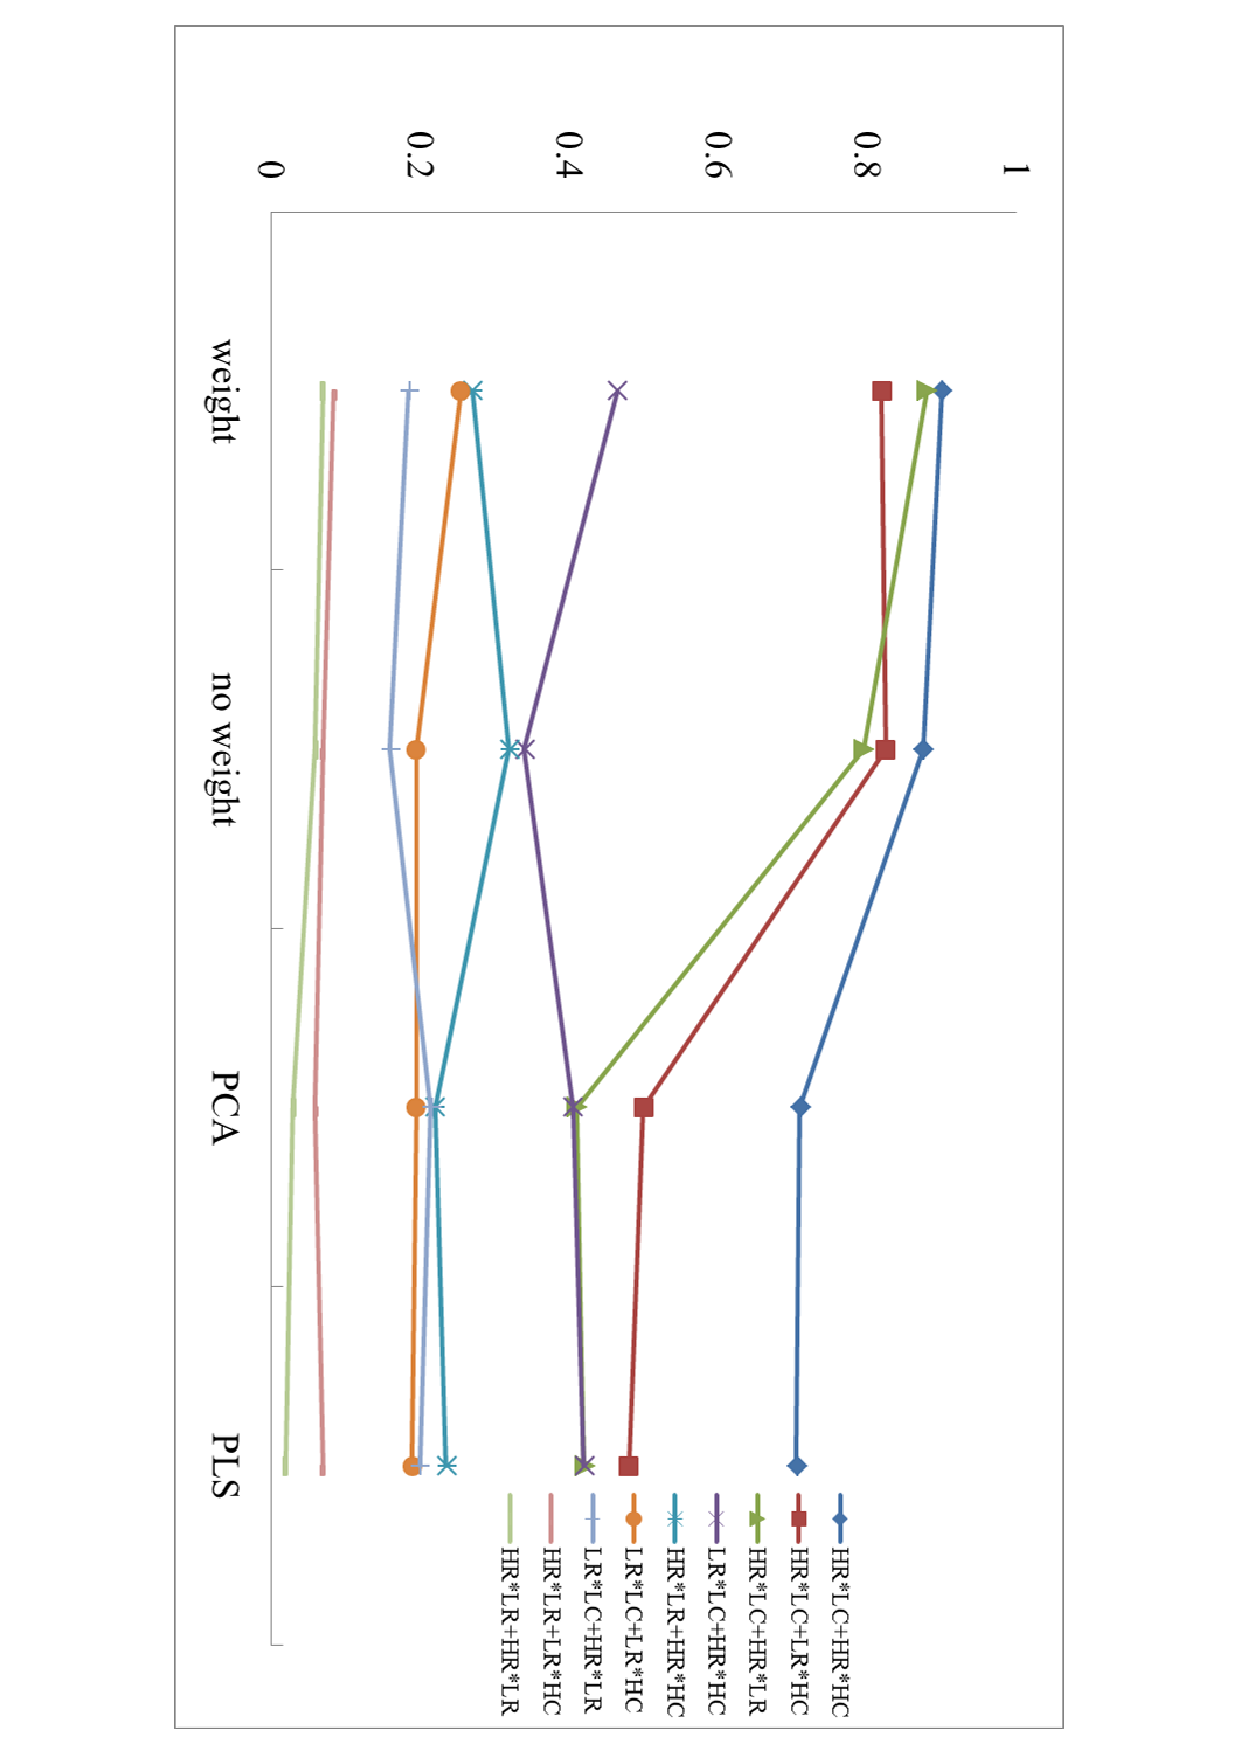
\includegraphics[scale=0.5,angle=90,trim=70 0 70 0, clip=true]{Model2}
            \caption{ALL combinations for Model 2}
        \end{figure}

        Model 2 is typical within gene interaction model. For Gene RBJ, there are 3 kinds of interactions, $HR\times LC$, $HR\times LR$ and $LC\times LR$. The rule of the power for the different kind is similar to Model 1: the larger the allele freq., the larger the power is. The higher the LD, the larger the power is. And the allele freq. is more important than the LD pattern. To sum up, when the interaction in Gene GRPC5B is fixed, the power follows the rule of $P_{HR\times LC}>P_{LC\times LR}>P_{HR\times LR}$. Similar to Gene RBJ, there are also 3 kinds of interactions in Gene GRPC5B: $HC\times HR$, $HC\times LR$ and $HR\times LR$. And the pattern of the power under the same type of Gene RBJ interaction is: $P_{HC\times HR}>P_{HC\times LR}>P_{HR\times LR}$.

        When the there are lots of common allele involved in the interactions, the model is easy to be detected. Also, under this situation, our method would perform better than PCA and PLS. But when lots of Low LD, rare allele involved, all the methods seems to have a very power to detect the interaction. Specifically, when the interaction in Gene RBJ is $L\times L$, PCA hand PLS have a larger power than our methods. (\textcolor{red}{One thing confuse me that weighted version performs better in $LR\times LC+HR\times HC$ than $LR\times LC+LR\times HC$})

    \subsection{Model 5: $Y=0.2\times(\theta_{11}\theta_{21}+\theta_{12}\theta_{22})+\epsilon$}
    
        \begin{figure}[htbp]
            \centering
            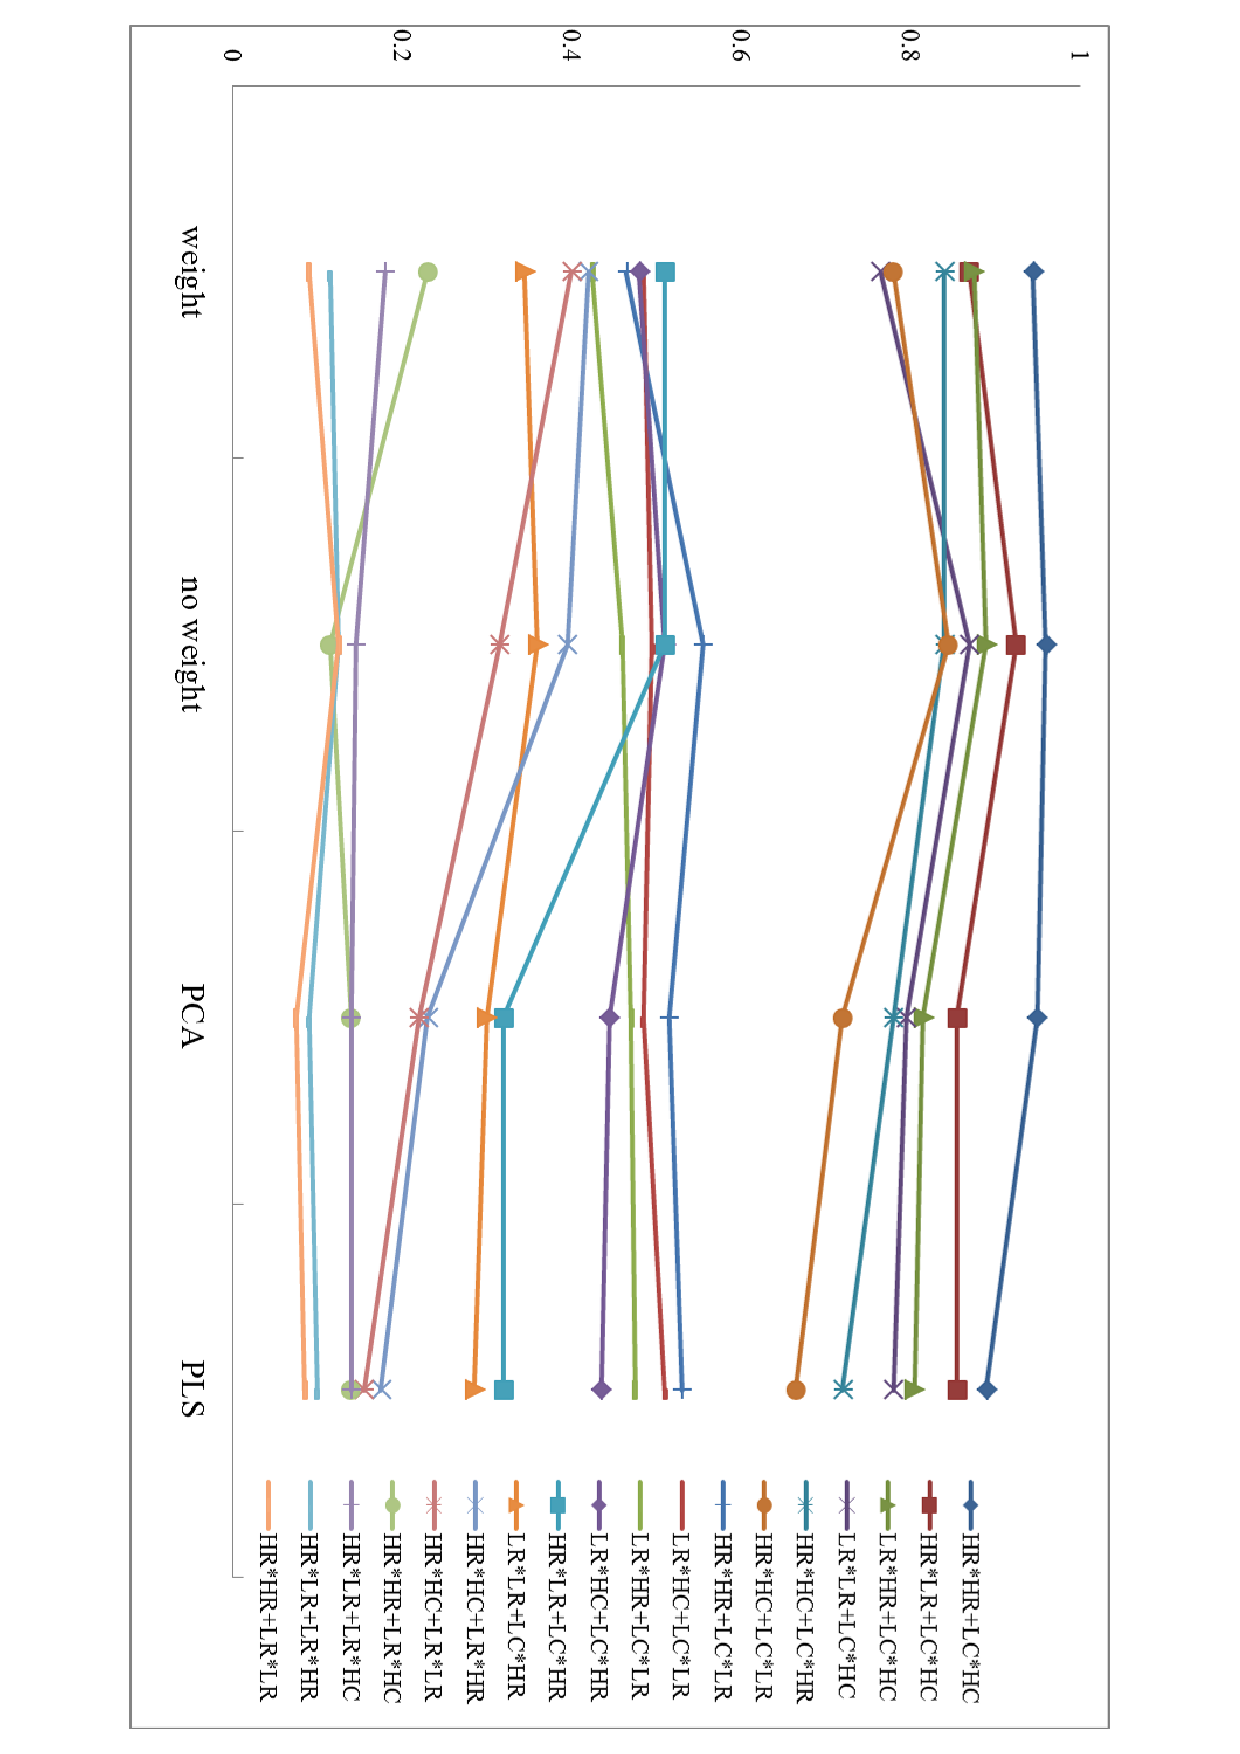
\includegraphics[scale=0.5,angle=90,trim=50 0 50 0, clip=true]{Model5}
            \caption{ALL combinations for Model 5}
        \end{figure}

        Model 5 is a typical between gene interaction model. From the figure we can see that allele freq. plays an more important role than the LD pattern. The top 4 combination all have the interaction term $LC\times HC$(since there is no SNP in Gene RBJ has the HC pattern. Otherwise, I believe that the biggest power should belong to the model which has the interaction term of $HC\times HC$). In the top 4 combinations, checking the other interaction term we can see that high LD will give us a better power: $P_{HR\times HR}>P_{HR\times LR}>P_{LR\times HR}>P_{LR\times LR}$. If we just go through the allele freq and LD pattern, we have the following rules: $P_{C\times C}>P_{C\times R}>P_{R\times R}$ and $P_{H\times H}>P_{H\times L}>P_{L\times L}$. The allele freq. is more important in determining the power.

        When we compare the power of weighted and no weight, we find out that when LC shows up, weighted would perform worse than the no weight version. In most case, our method would gain a higher power than PCA and PLS. The only bad performance shows up in the case  $LR\times HR+LC\times LR$. I think the reason is that 3 over 4 SNPs are in low LD and most of them are rare allele.
    
    \subsection{Model 3 and Model 4}
        \begin{figure}[htbp]
            \centering
            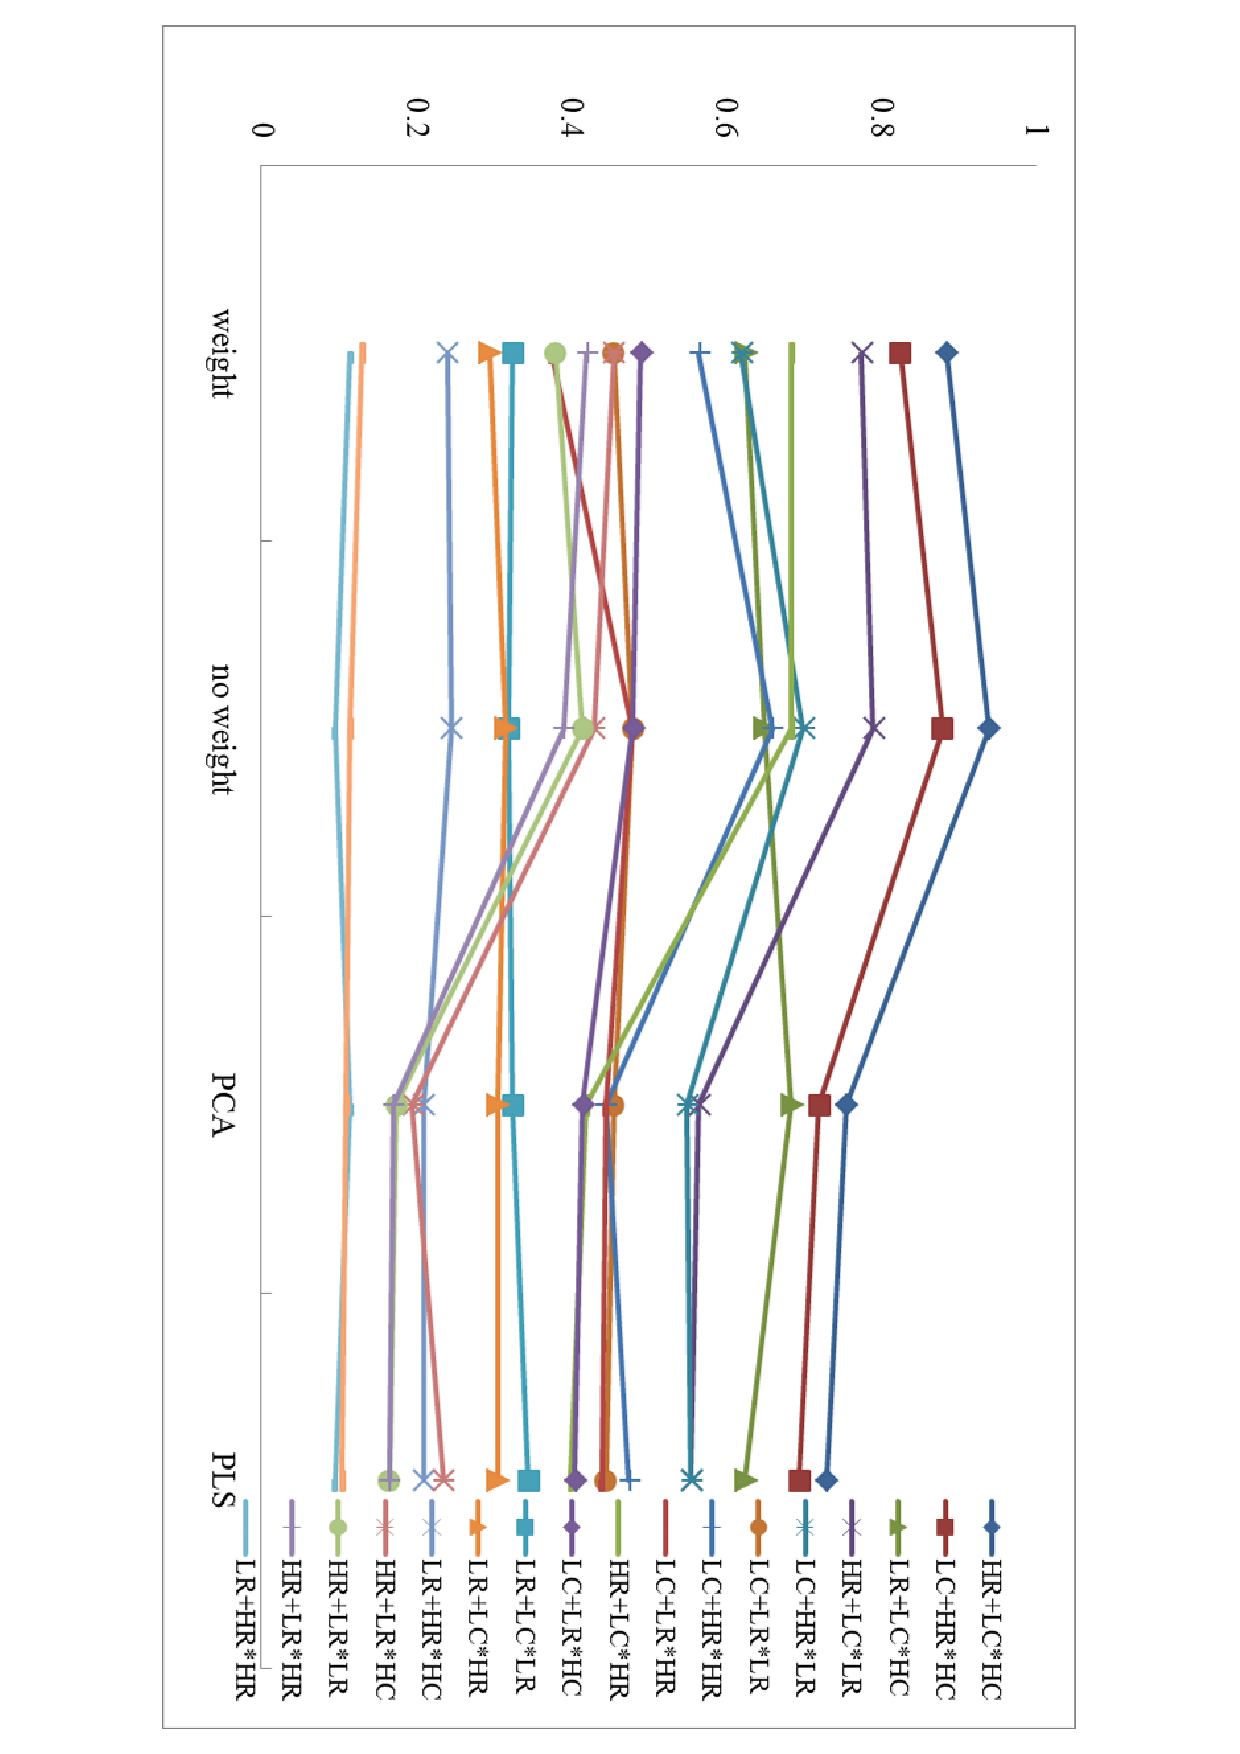
\includegraphics[scale=0.5,angle=90,trim=50 0 50 0, clip=true]{Model3}
            \caption{ALL combinations for Model 3}
        \end{figure}
        \begin{figure}[htbp]
            \centering
            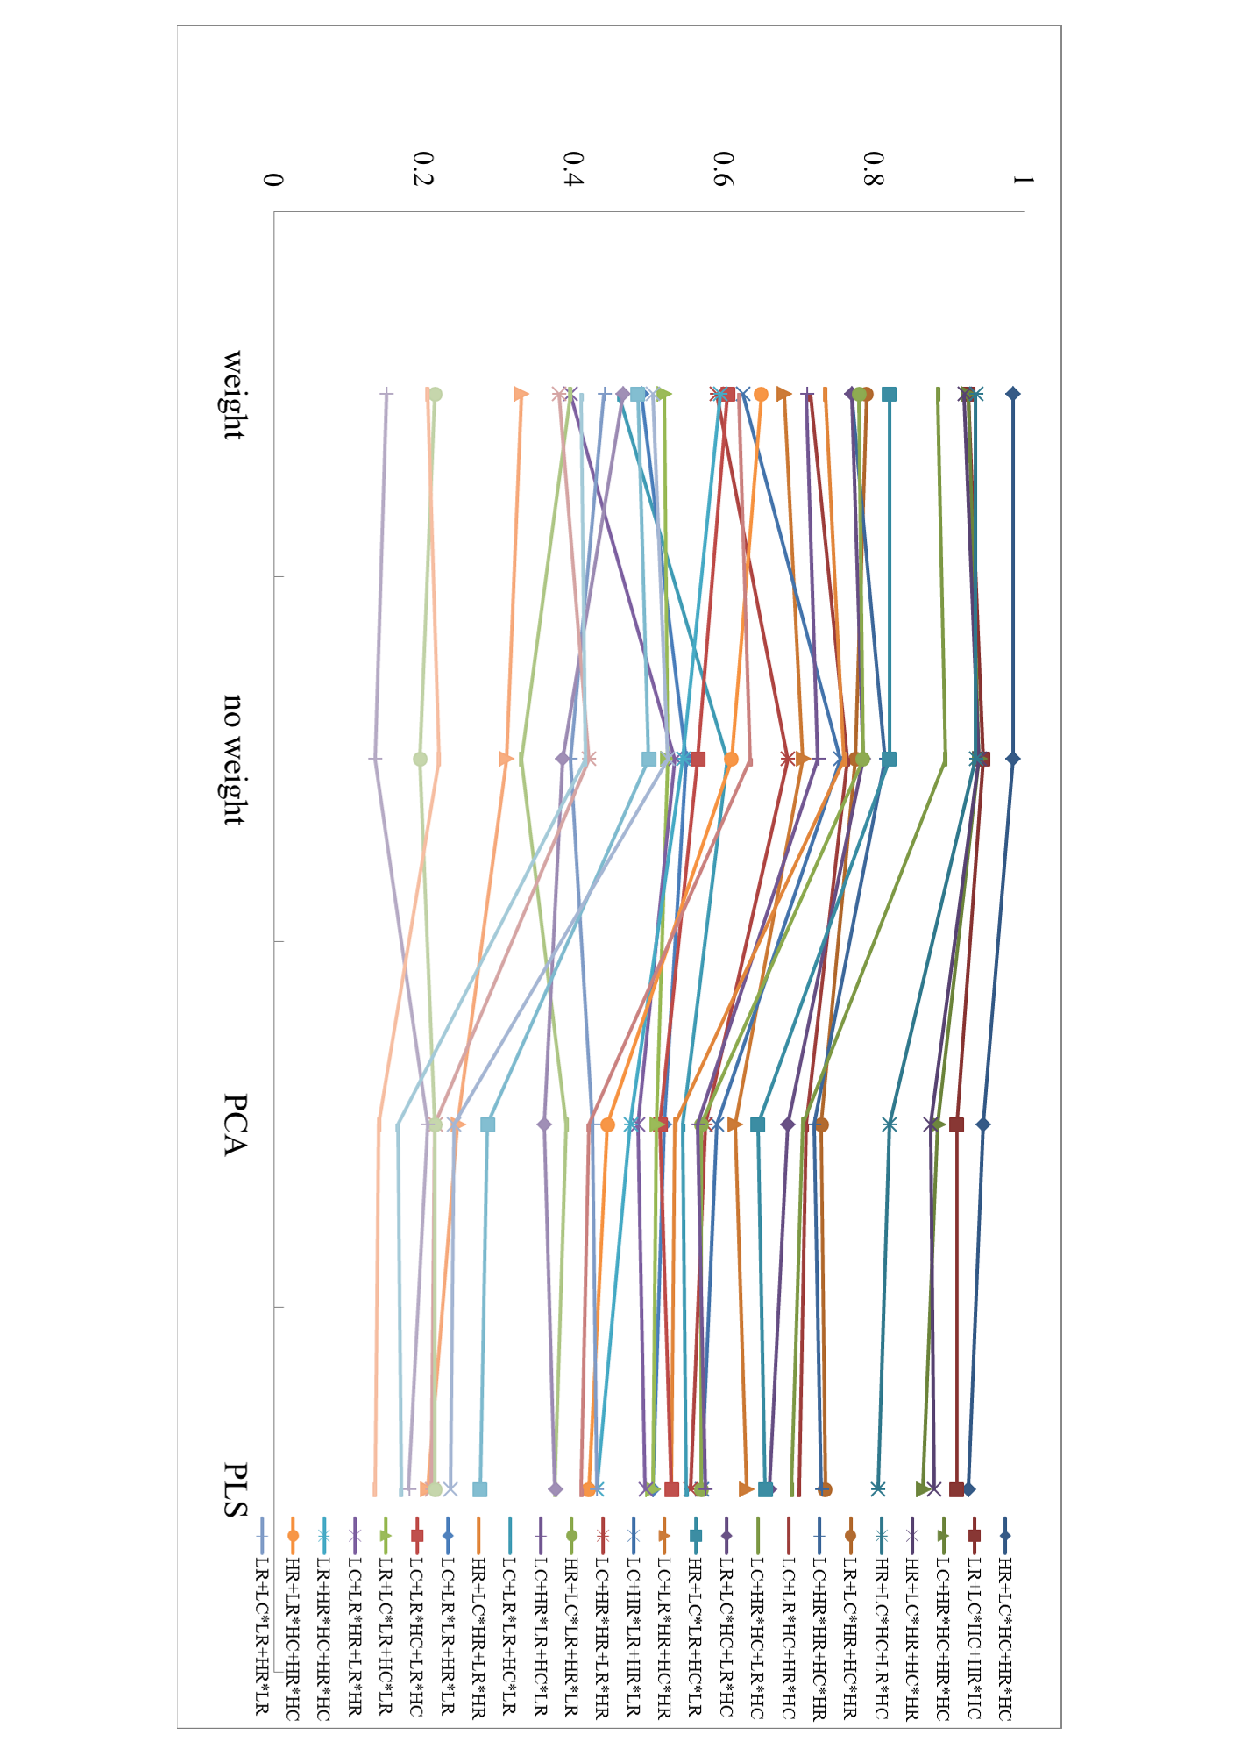
\includegraphics[scale=0.5,angle=90,trim=70 0 70 0, clip=true]{Model4}
            \caption{ALL combinations for Model 4}
        \end{figure}
        
        Model 3 is a risk model consider both main effect and between gene interaction. Model 4 add an within gene interaction ($\theta_{21}\theta_{22}$) based on Model 3. It is hard to directly find the pattern of power of the two model. But based on the observation from previous models, we can found the following rules:  Both for the main effect and the interaction effect, the bigger the allele freq, the larger the power is. The higher the LD, the larger the power is. Also, similar to previous rules: the allele freq. seems more important than the LD pattern.
        
        Compare to other method, we can see in most cases our methods are better than PCA and PLS. But when $\theta_{11}$ is the LR type and $\theta_{12}$ is the LC type, our methods perform worse than PCA and PLS.
        
        



\end{document}
